\documentclass[UTF8,a1paper,twoside,11pt]{article}
\usepackage{./package/constar_package_font} %Constar font Package
\usepackage[explicit,clearempty]{titlesec}
\usepackage{./package/constar_package_general} %Constar general Package
\usepackage{./package/constar_package_term} %Constar term Package
\usepackage{indentfirst} %Constar term Package
\setlength{\parindent}{54pt}
\usetikzlibrary{shapes,positioning}
\usetikzlibrary{intersections,arrows,decorations.pathmorphing,backgrounds,positioning,fit,petri,shapes.geometric,shapes.misc,calc,graphs,circuits.logic.us} %TZK画图常用库
\setwatermarktext{\hspace{1em}} %Remove watermark brough by constar_term_pakage
\usepackage{booktabs} 		%绘图
\usepackage{pgfplots} 		%绘图
\geometry{
   left=23mm,  %% or inner=23mm
   right=18mm, %% or outer=18mm
   %top=63mm, bottom=16mm}
   top=170mm, bottom=16mm}

%% Command to hold chapter illustration image
\newcommand\chapterillustration{}
\renewcommand{\figurename}{图.}
\renewcommand{\tablename}{表.}

\renewcommand{\baselinestretch}{1}
\setlength{\baselineskip}{100pt}
\setlength{\lineskiplimit}{1pt}
\setlength{\parskip}{0pt}


%%% Define how the chapter title is printed
%\titleformat{\chapter}{\centering\Huge\bf}{}{0pt}{
%%% Background image at top of page
%\ThisULCornerWallPaper{1}{\chapterillustration}
%%% Draw a semi-transparent rectangle across the top
%\tikz[overlay,remember picture]
%  \fill[LightSalmon1,opacity=.7]
%  (current page.north west) rectangle 
%  ([yshift=-3cm] current page.north east);
%  %% Check if on an odd or even page
%  \strictpagecheck\checkoddpage
%  \ifoddpage{
%    \ThisLRCornerWallPaper{.35}{fern_mo_01}
%    \begin{tikzpicture}[overlay,remember picture]
%    \node[anchor=south west,
%      xshift=20mm,yshift=-30mm,
%      font=\sffamily\bfseries\huge] 
%      at (current page.north west) 
%      {\chaptername\ \thechapter};
%    \node[fill=Sienna!80!black,text=white,
%      font=\Huge\bfseries, 
%      inner ysep=12pt, inner xsep=20pt,
%      rounded rectangle,anchor=east, 
%      xshift=-20mm,yshift=-30mm] 
%      at (current page.north east) {#1};
%    \end{tikzpicture}
%  }
%  \else {
%    \ThisLLCornerWallPaper{.35}{fern_mo_01}
%    \begin{tikzpicture}[overlay,remember picture]
%    \node[anchor=south east,
%      xshift=-20mm,yshift=-30mm,
%      font=\sffamily\bfseries\huge] 
%      at (current page.north east)
%      {\chaptername\ \thechapter};
%    \node[fill=Sienna!80!black,text=white,
%      font=\Huge\bfseries,
%      inner sep=12pt, inner xsep=20pt,
%      rounded rectangle,anchor=west,
%      xshift=20mm,yshift=-30mm] 
%      at ( current page.north west) {#1};
%    \end{tikzpicture}
%  }
%  \fi
%}
%%% Define how the chapter title is printed
%\titleformat{name=\chapter,numberless}{}{}{0pt}{
%%% Draw a semi-transparent rectangle across the top
%\tikz[overlay,remember picture]
%  \fill[LightSalmon1,opacity=.7]
%  (current page.north west) rectangle 
%  ([yshift=-3cm] current page.north east);
%  %% Check if on an odd or even page
%  \strictpagecheck\checkoddpage
%  \ifoddpage{
%    \begin{tikzpicture}[overlay,remember picture]
%    \node[fill=Sienna!80!black,text=white,
%      font=\Huge\bfseries, 
%      inner ysep=12pt, inner xsep=20pt,
%      rounded rectangle,anchor=east, 
%      xshift=-20mm,yshift=-30mm] 
%      at (current page.north east) {#1};
%    \end{tikzpicture}
%  }
%  %% On even pages, "logo" image at lower left
%  %% corner; Chapter number printed near outer
%  %% edge (near the right); chapter title printed
%  %% near spine edge (near the left).
%  \else {
%    \begin{tikzpicture}[overlay,remember picture]
%    \node[fill=Sienna!80!black,text=white,
%      font=\Huge\bfseries,
%      inner sep=12pt, inner xsep=20pt,
%      rounded rectangle,anchor=west,
%      xshift=20mm,yshift=-30mm] 
%      at ( current page.north west) {#1};
%    \end{tikzpicture}
%  }
%  \fi
%}
%\titlespacing*{\chapter}{0pt}{0pt}{135mm}
%\titlespacing*{name=\chapter,numberless}{0pt}{0pt}{50mm}

%% Set the uniform width of the colour box
%% displaying the page number in footer
%% to the width of "99"
\newlength\pagenumwidth
\settowidth{\pagenumwidth}{99}

%%% Define style of page number colour box
%\tikzset{pagefooter/.style={
%anchor=base,font=\sffamily\bfseries\small,
%text=white,fill=Sienna!80!black,text centered,
%text depth=17mm,text width=\pagenumwidth}}

%% Concoct some colours of our own
%\definecolor[named]{GreenTea}{HTML}{CAE8A2}
%\definecolor[named]{MilkTea}{HTML}{C5A16F}
%\definecolor[named]{CoverRed}{RGB}{192,0,0}
%\definecolor[named]{contentgray}{RGB}{234,234,234}
\definecolor[named]{titleblue1}{RGB}{25,25,112}
\definecolor[named]{titleblue2}{RGB}{65,105,225}

%%%%%%%%%%%
%%%% Re-define running headers on non-chapter pages
%%%%%%%%%%%
%\fancypagestyle{headings}{%
%  \fancyhf{}   % Clear all headers and footers first
%  %% Right headers on odd pages
%  \fancyhead[RO]{%
%    %% First draw the background rectangles
%    \begin{tikzpicture}[remember picture,overlay]
%    \fill[MilkTea!25!white] (current page.north east) rectangle (current page.south west);
%    \fill[white, rounded corners] ([xshift=-10mm,yshift=-20mm]current page.north east) rectangle ([xshift=15mm,yshift=17mm]current page.south west);
%    \end{tikzpicture}
%    %% Then the decorative line and the right mark
%    \begin{tikzpicture}[xshift=-.75\baselineskip,yshift=.25\baselineskip,remember picture,    overlay,fill=GreenTea,draw=GreenTea]\fill circle(3pt);\draw[semithick](0,0) -- (current page.west |- 0,0);\end{tikzpicture} \sffamily\itshape\small\nouppercase{\rightmark}
%  }
%
%  %% Left headers on even pages
%  \fancyhead[LE]{%
%    %% Background rectangles first
%    \begin{tikzpicture}[remember picture,overlay]
%    \fill[MilkTea!25!white] (current page.north east) rectangle (current page.south west);
%    \fill[white, rounded corners] ([xshift=-15mm,yshift=-20mm]current page.north east) rectangle ([xshift=10mm,yshift=17mm]current page.south west);
%    \end{tikzpicture}
%    %% Then the right mark and the decorative line
%    \sffamily\itshape\small\nouppercase{\leftmark}\ 
%    \begin{tikzpicture}[xshift=.5\baselineskip,yshift=.25\baselineskip,remember picture, overlay,fill=GreenTea,draw=GreenTea]\fill (0,0) circle (3pt); \draw[semithick](0,0) -- (current page.east |- 0,0 );\end{tikzpicture}
%  }
%
%  %% Right footers on odd pages and left footers on even pages,
%  %% display the page number in a colour box
%  \fancyfoot[RO,LE]{\tikz[baseline]\node[pagefooter]{\thepage};}
%  \renewcommand{\headrulewidth}{0pt}
%  \renewcommand{\footrulewidth}{0pt}
%}

%%%%%%%%%%
%%% Re-define running headers on chapter pages
%%%%%%%%%%
\fancypagestyle{plain}{%
  %% Clear all headers and footers
  \fancyhf{}
  %% Right footers on odd pages and left footers on even pages,
  %% display the page number in a colour box
  \fancyfoot[RO,LE]{\tikz[baseline]\node[pagefooter]{\thepage};}
  \renewcommand{\headrulewidth}{0pt}
  \renewcommand{\footrulewidth}{0pt}
}

%\titleformat{\subsection}{\left}{}{1em}{0pt}[0pt]

%\titleformat{name=\section, numberless}{\LARGE\bfseries\flushleft}{}{1em}{0pt} % 正文的section标题格式
%\titleformat{name=\section}{\LARGE\bfseries\flushleft}{}{1em}{0pt} % 正文的section标题格式
\begin{document}

%\titleformat{\section*}{\large\bfseries}{\thesection}{1em}{} % 正文前的section标题格式
%\titleformat{\section}[block] {first}{label}{0pt}{\textbf{#1}}[trailer] % all versions
%\titleformat{\section}[block,numberless]{first}{label}{0pt}{#1}[trailer] % starred version
\newcommand{\titlephotopositionx}{0.75}
\newcommand{\titlephotopositiony}{0.03}
\newcommand{\titlephotowidth}{0.2}
\newcommand{\titlephotoheight}{0.3}

\begin{tikzpicture}[remember picture,overlay]
\fill[titleblue1] (current page.north west) rectangle ([yshift=-0.2*0.9\paperheight]current page.north east); %顶部蓝色背景1
\fill[titleblue2] ([yshift=-0.2*0.9*\paperheight]current page.north west) rectangle ([yshift=-0.2\paperheight]current page.north east);%顶部蓝色背景2
\fill[titleblue1] (current page.south west) rectangle ([yshift=0.05\paperheight]current page.south east);%底部蓝色背景
%\node[below right, yshift=-0.2*0.3\paperheight, xshift=0.1*\paperwidth, minimum width = 6cm, minimum height = 1{em}, align=left] (maintitle) at (current page.north west) {\fontyahei{\yihao{\textcolor{white}{梅钢透平电液伺服冗余改造}}}};
\node[below right, yshift=-0.2*0.3\paperheight, xshift=18mm, minimum width = 6cm, minimum height = 1{em}, align=left] (maintitle) at (current page.north west) {\fontyahei{\tehao{\textcolor{white}{金陵石化一号二号双抽机组DEH控制系统}}}};
\node[below right, yshift=-0.2*0.3\paperheight-3cm, xshift=18mm, minimum width = 6cm, minimum height = 1cm, align=left] (keyword) at (current page.north west) {\fontyahei{\yihao{\textcolor{white}{关键词:  \textcolor{yellow}{上汽、双抽、DEH、Micronet TMR, 金陵石化}}}}};
\node[anchor=north west, inner sep=0pt, outer sep=0pt] at ([yshift=-1*\titlephotopositiony*\paperheight, xshift=\titlephotopositionx*\paperwidth]current page.north west) {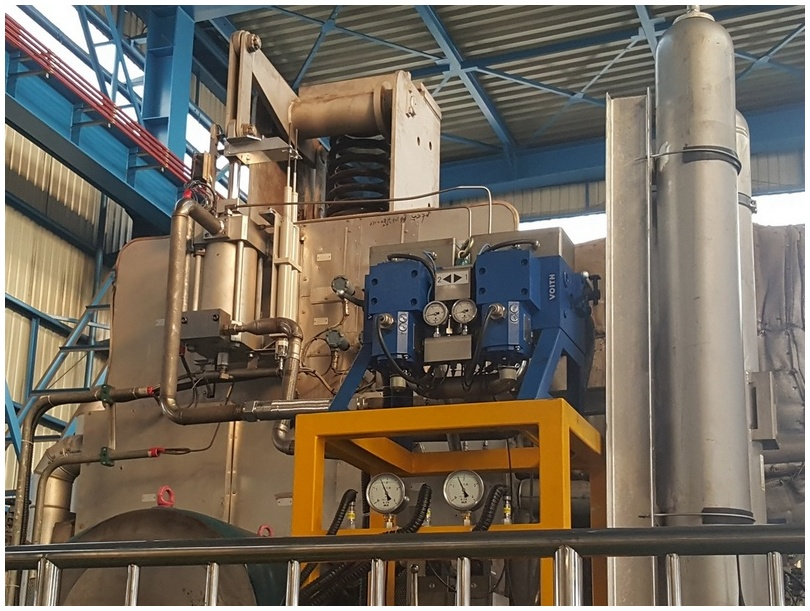
\includegraphics[width=12cm]{titlephoto.jpg}};
\end{tikzpicture}\par

\renewcommand{\baselinestretch}{1} %字体设为一号, 调整行间距为1.5倍
\setlength{\baselineskip}{42pt}
\setlength{\lineskiplimit}{1pt}
\setlength{\parskip}{0pt}

{\fontyahei{\yihao{中石化金陵石化热电厂的两台50MW双抽热电联产机组是上海汽轮机厂的50MW双抽机组,最初安装是纯机械液压调速器,存在控制精度差和自动化程度低等缺点。控之星于2002年和2003年分别对一号机组和二号机组进行了汽轮机数字电液控制系统(DEH)改造, DEH的硬件核心是Woodward公司的三冗余控制平台Micronet TMR, 软件算法核心是热电牵联解耦算法,电液伺服结构采用低压透平油系统, 成功地使发电机组同时稳定地自动控制两路抽汽压力和机组负荷。将近二十年来,两台双抽机组稳定而可靠地为金陵石化输送的源源不断的蒸汽和供电,用二十年的实际业绩证明了控之星自动化优秀的热电联产控制算法和可靠的工程质量}}\par

\begin{multicols}{2}
\section*{{\fontyahei{\yihao{基本数据}}}}
\par
\begin{itemize}
	\item 汽轮机制造厂:上海汽轮机厂
	\item 负荷: 60MW
	\item 类型: 双抽
	\item 控制油: 低压透平油
	\item 控制系统: Micronet TMR
	\item 改造日期: 2001年
\end{itemize}




为提高动力机组的安全性, 大多数的安全措施集中在了电子控制部分,例如采用冗余控制模板, 甚至冗余传感器等。但是,由于机组控制是一个整体,即使电控部分冗余度再高,电液伺服驱动部分仍然是控制系统中的单点,并且由于此环节是电液转换接口, 所以结构复杂、系统精密、对油质要求高,恰好是电液控制系统中容易出故障的环节。所以,提高电液伺服驱动部分的可靠性对提高机组安全性有重大意义。\par
梅钢新三号透平鼓风机组是梅钢生产中的关键动力设备, 恰好曾经发生电液伺服部件故障,导致机组停机。所以,解决新三号机组电液伺服冗余的问题迫在眉睫。同时,由于电液伺服冗余系统结构复杂、系统精密、冗余措施要兼顾电子和液压两个方面、实施难度大,在世界范围内成功实施的项目都不多,在国内更是罕见,所以此改造项目在电液伺服冗余控制领域有一定的探索意义。\par

\section*{改造前系统}
改造前的电液伺服驱动部分由电子控制系统信号(4-20mA)、福伊特位阀(Way Valve)、反馈装置(MLDT)组成, 还包括机组的供油和排油管路。位阀接收控制系统的阀位指令(4-20mA), 位阀进行指令与阀位反馈比较,输出控制油控制动力油缸. 系统控制效果良好,但是所有部件都是一套,任何部件故障会造成机组停机, 改造前系统原理如图 \ref{fig:servo_before} 所示。\par

\section*{改造方案}
%\raggedbottom
\subsection*{方案概述}
改造方案采用福伊特公司的WSM装置(WSM是Voith公司专门设计的一体式冗余装置, 包括两套完全独立电液伺服位阀(Way Valve)、液压冗余表决部件、以及必要的仪表和手动切换装置等)、并配置两套油动机位置反馈装置(MLDT)、并且从控制器引出双路阀位控制指令,供电系统也改造为完全独立的两路24VDC供电。两套电液伺服位阀接收独立的控制指令(4-20mA), 两路出口控制油路再进行液压冗余表决, 直接驱动油缸。系统从控制指令、电液伺服位阀、油缸位置传感器、系统供电完全冗余,任何部件故障不停机。\par
为了更好的监控冗余装置的工作状态,虽然不是必需,但改造方案还包括了一套独立的冗余装置监控系统。监控系统以PLC为核心, 配备专门设计的双路供油切断阀及专门设计的切断液压块,不仅可以显示每路供油压力、控制油压力及冗余表决后的控制油压,而且可以在需要的时候切断供油油压,并且具有报警等功能。此监控系统以PLC控制器为核心,独立运行,是冗余装置的辅助系统,即使此PLC故障或失电,也不会影响机组伺服冗余装置工作。改造后的系统原理如图\ref{fig:servo_after}所示。\par

\subsection*{WSM冗余装置}
%\raggedbottom
系统的主要部件是福伊特WSM冗余装置,包括两套完全独立电液伺服位阀(Way Valve)、液压冗余表决部件、必要的仪表和手动切换装置等, 如图\ref{fig:wsm}所示。\par
\end{multicols}

\newpage
\newgeometry{
   left=18mm,  %% or inner=23mm
   right=18mm, %% or outer=18mm
   top=23mm, bottom=16mm,
   headheight=\baselineskip,
   headsep=7mm,
   footskip=10mm
}
%\newgeometry{
%   left=18mm,  %% or inner=23mm
%   right=18mm, %% or outer=18mm
%   top=63mm, bottom=12mm}
\headfootnormalbody
\begin{tikzpicture}[remember picture,overlay]
\fill[titleblue1] (current page.south west) rectangle ([yshift=0.05\paperheight]current page.south east);%底部蓝色背景
\end{tikzpicture}

\begin{figure}[H]
\begin{center}
\begin{tikzpicture}[ >=stealth, very thick]

		%主要部件尺寸
		\def\hsep{4cm};
		\def\vsep{1cm};
		\def\minwidth{2cm};
		\def\minheight{1cm};
		\tikzstyle{block}=[rectangle, rounded corners=2mm, minimum width =\minwidth, minimum height = \minheight, thick, draw=black!50, font= \rmfamily]
		%\draw[help lines,very thin, black!20] (0,0) grid [step=0.5cm] (14,4);	
		\node[coordinate] (controller) at (0, 0) {};
		\node[block] (voith)  [right= 0.5*\hsep of controller.east] {Voith位阀};
		\node[block] (cylinder) [right= \hsep of voith.east] {油缸};
		\node[coordinate] (valve) [right= 0.5*\hsep of cylinder.east] {};
		\node[block] (lvdt)  at (voith.north east) [above right = \vsep and 0.5*\hsep, anchor=center] {MLDT};

		\draw[->,black!50] (controller) -- node[above,black]{调门指令} node[below,black]{4-20mA} (voith);		
		\draw[->,black!50] (voith) -- node[above,black]{控制油压} (cylinder);		
		\draw[->,black!50] (cylinder.north) |- node[above,black,near end]{位置反馈} (lvdt.east);
		\draw[->,black!50] (lvdt.west) -| node[above,black, near start]{位置反馈} (voith.north);
		\draw[->,black!50] (cylinder.east) -- node[above,black]{驱动调门} (valve);

		%\draw[->,black!50] (cylinder.east) -- node[above,black]{驱动调门} (valve.west);
		%\draw[->,black!50] (lvdt.west) -| node[near start, below]{位置反馈} (voith.north);
%		\draw[->,black!50] (lvdt.west) to [out=135, in=95] (voith.north);
																	
\end{tikzpicture}
\caption{改造前的伺服系统示意图}
\label{fig:servo_before}
\end{center}
\end{figure} 

%%\raggedbottom

\begin{figure}[H]
\begin{center}
\begin{tikzpicture}[ >=stealth, very thick ]
		\def\hsep{4cm};
		\def\vsep{1cm};
		\def\minwidth{2cm};
		\def\minheight{1cm};
		\def\sep{1.5cm};
		\def\framewidth{6.8cm};
		\def\frameheight{3cm};
		\tikzstyle{block}=[rectangle, rounded corners=2mm, minimum width =\minwidth, minimum height = \minheight, thick, draw=black!50, font= \rmfamily]

		\node[coordinate] (controller1) at (0, 0) {};
		\node[block] (voith1)  [right= 0.75*\hsep of controller1.east] {Voith位阀A};
		\node[block] (lvdt1)  at (voith1.north east) [above right = \vsep and 0.5*\hsep, anchor=center] {MLDT A};

		\node[coordinate] (controller2) at (0, -\sep) {};
		\node[block] (voith2)  [right= 0.75*\hsep of controller2.east] {Voith位阀B};
		\node[block,minimum height= 2.5*\minheight,minimum width= 0.5*\minwidth] (vote) at (voith1.east) [below right= 0.75*\vsep and 0.75*\hsep, anchor=center] {表决};
		\node[block] (cylinder) at (vote.east) [right= 1.5*\vsep] {油缸};
		\node[coordinate] (valve) [right= 0.5*\hsep of cylinder.east] {};
		\node[block] (lvdt2)  at (voith2.south east) [below right = \vsep and 0.5*\hsep, anchor=center] {MLDT B};
		\node[coordinate] (votepoint1)  at ($(vote.north west)!(voith1.east)!(vote.south west)$) {};
		\node[coordinate] (votepoint2)  at ($(vote.north west)!(voith2.east)!(vote.south west)$) {};
		\node[rectangle,minimum width=\framewidth, minimum height=\frameheight, draw, dashed, black!50, anchor=center] (framecenter) at (vote.west) [left=0.5*\hsep, anchor= center] {};
		\node (text) at (framecenter.south west) [below left =0.3*\hsep and 0.3*\hsep, anchor= center] {Vioth WSM};

		\draw[->,black!50] (controller1) -- node[above,black]{调门指令A} node[below,black]{4-20mA} (voith1);		
		\draw[->,black!50] (controller2) -- node[above,black]{调门指令B} node[below,black]{4-20mA} (voith2);		
		\draw[->,black!50] (cylinder.north) |- node[above,black,near end]{位置反馈} (lvdt1.east);
		\draw[->,black!50] (lvdt1.west) -| node[above,black, near start]{位置反馈} (voith1.north);
		\draw[->,black!50] (cylinder.south) |- node[above,black,near end]{位置反馈} (lvdt2.east);
		\draw[->,black!50] (lvdt2.west) -| node[above,black, near start]{位置反馈} (voith2.south);
		\draw[->,black!50] (cylinder.east) -- node[above,black]{驱动调门} (valve);
		\draw[->,black!50] (voith1.east) -- node[above,black]{控制油压A} (votepoint1);		
		\draw[->,black!50] (voith2.east) -- node[above,black]{控制油压B} (votepoint2);		
		\draw[->,black!50] (vote.east) -- node[above,black]{控制油压} (cylinder);		
		\draw[->,black!50] (text) ->  (framecenter.south west);		
\end{tikzpicture}
\caption{改造后的伺服系统示意图}
\label{fig:servo_after}
\end{center}
\end{figure} 

\begin{multicols}{2}
\subsection*{油动机位置反馈装置}
 测量油动机位置反馈装置采用两支德国Balluff公司的MLDT油缸位置传感器,而不是普通的拉杆式LVDT, 因为MDLT采用磁致伸缩原理,能够通过机械变形提供绝对位置信息、精度高、而且底部集成信号调理电路,安装方便。并且为了保证安装精度,专门设计了双冗余MLDT的安装支架,如图\ref{fig:mldt}所示。\par



\begin{figure}[H]
\begin{center}
%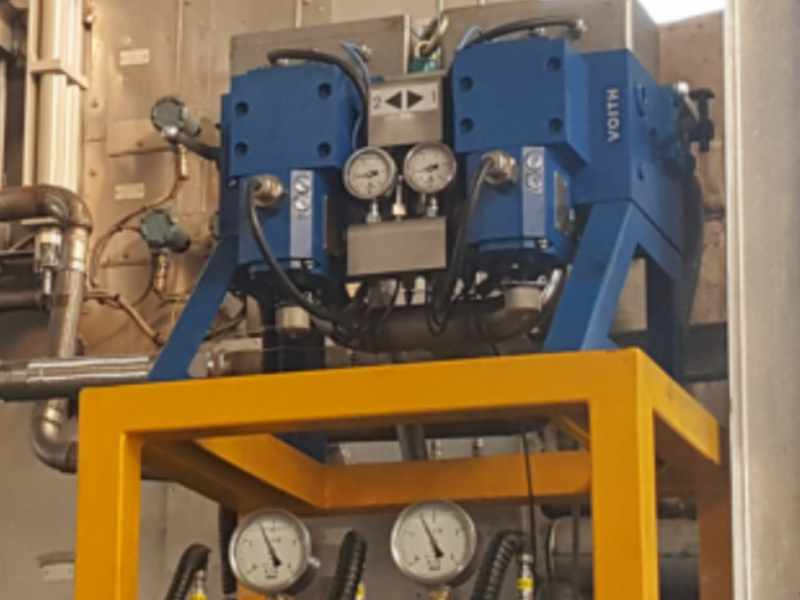
\includegraphics[angle=0,width=0.4\textwidth]{wsm.jpg}
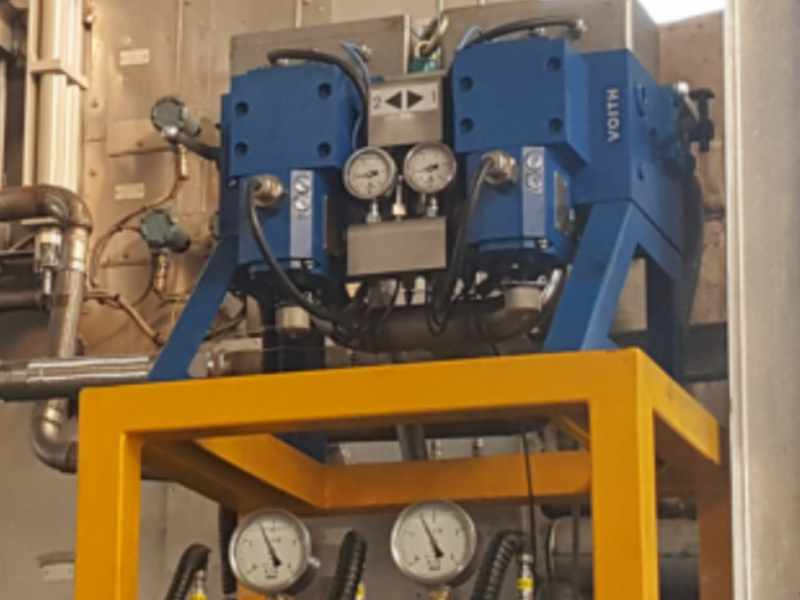
\includegraphics[angle=0,width=0.9\columnwidth]{wsm.jpg}
\caption{Voith WSM冗余装置}
\label{fig:wsm}
\end{center}
\end{figure}


\begin{figure}[H]
\begin{center}
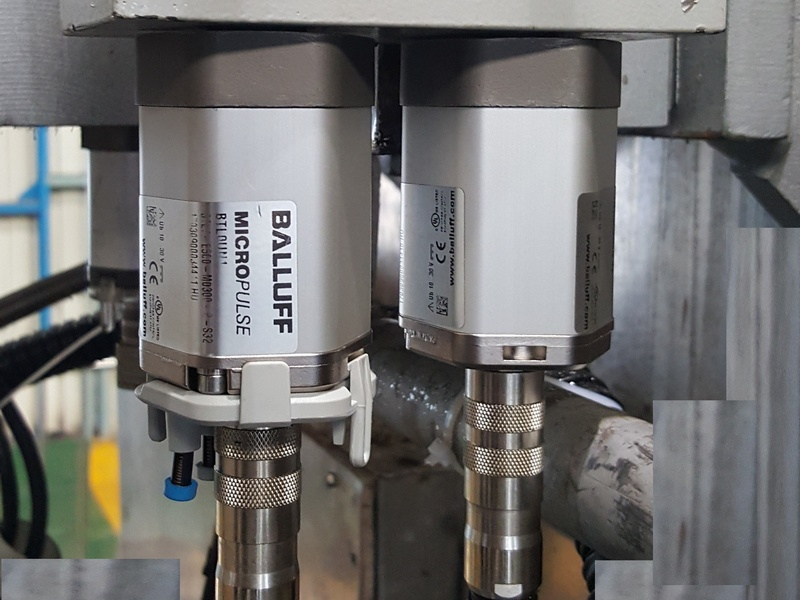
\includegraphics[angle=0,width=0.9\columnwidth]{mldt.jpg}
\caption{双冗余MLDT位置反馈组件}
\label{fig:mldt}
\end{center}
\end{figure}

\subsection*{冗余装置监控系统}
冗余装置的监控系统并不是必需的,但是可以实时监控冗余系统内部参数。系统采用以西门子PLC为核心的监控系统,采集两路供油油压、两路控制油压和冗余表决后的油压,显示在HMI触摸屏上。监控装置还可以在必要的时候单独控制每路电磁阀。同时, 系统专门设计了集成液压阀块,方便地实现了电磁阀的安装、手动油路控制和必要的液压参数采集功能。液压集成装置如图\ref{fig:hydrau_block}所示,监控系统画面如图\ref{fig:hmi}所示。\par

\begin{figure}[H]
\begin{center}
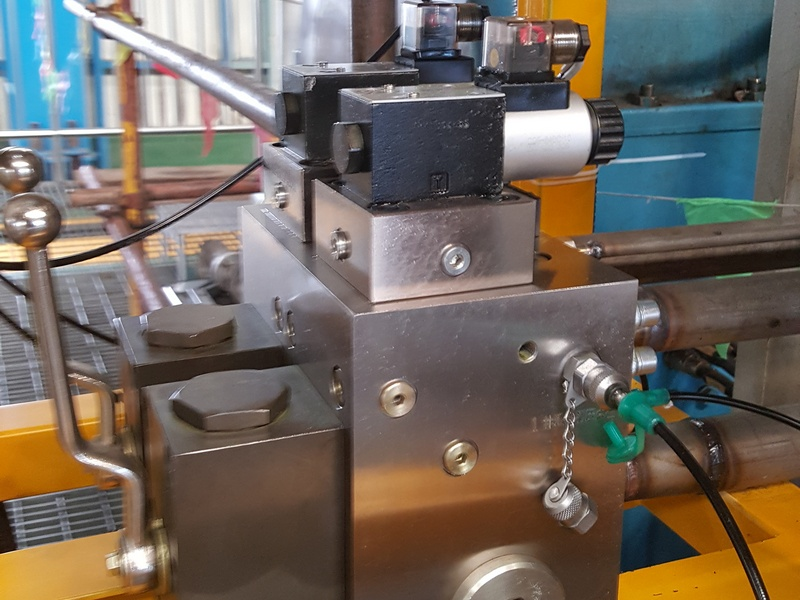
\includegraphics[angle=0,width=0.9\columnwidth]{hydrau_block.jpg}
\caption{专门设计的液压集成装置}
\label{fig:hydrau_block}
\end{center}
\end{figure}

%\begin{figure}[H]
%\begin{center}
%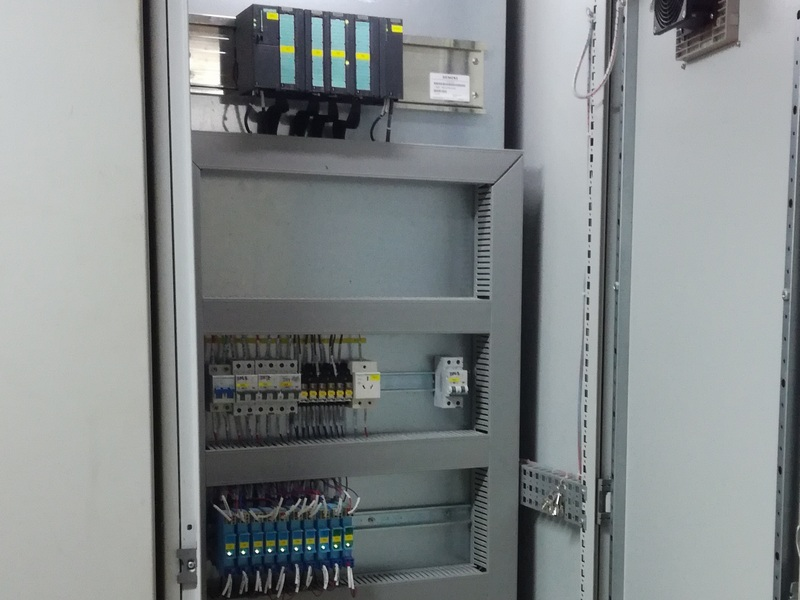
\includegraphics[angle=0,width=0.9\columnwidth]{plc.jpg}
%\caption{冗余装置监控机柜}
%\label{fig:plc}
%\end{center}
%\end{figure}

\begin{figure}[H]
\begin{center}
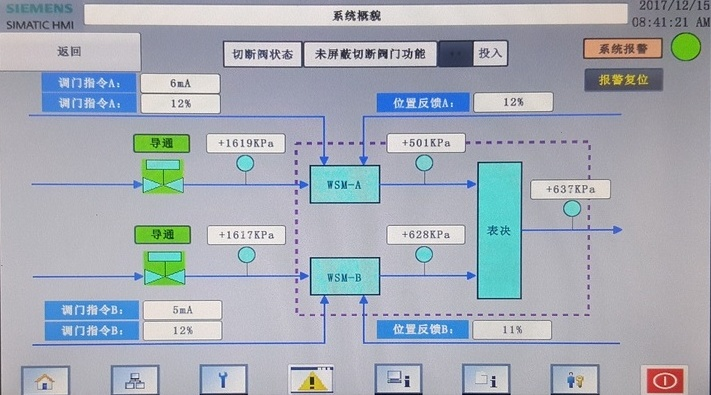
\includegraphics[angle=0,width=0.9\columnwidth]{hmi.jpg}
\caption{监控系统画面}
\label{fig:hmi}
\end{center}
\end{figure}

\begin{tikzpicture}[remember picture,overlay]
\fill[titleblue1] (current page.south west) rectangle ([yshift=0.05\paperheight]current page.south east);%底部蓝色背景
\end{tikzpicture}
\section*{项目施工}
%\raggedbottom
因为伺服机构结构复杂,系统精密,加上MLDT位置传感器对安装精度要求高,所以工程施工是此项目的一个关键环节。为保证项目成功,从安装的多个方面采取了措施。\par
油路管道改造方面,根据现有的液压管路,合理布局,精确的设计改造后油路, 并考虑管道的振动等因素,加装中间软管, 减小振动对可靠性的影响。同时,为了方便安装WSM冗余装置和液压集成装置,专门设计了装置安装支架等装置。\par
%\begin{figure}[H]
%\begin{center}
%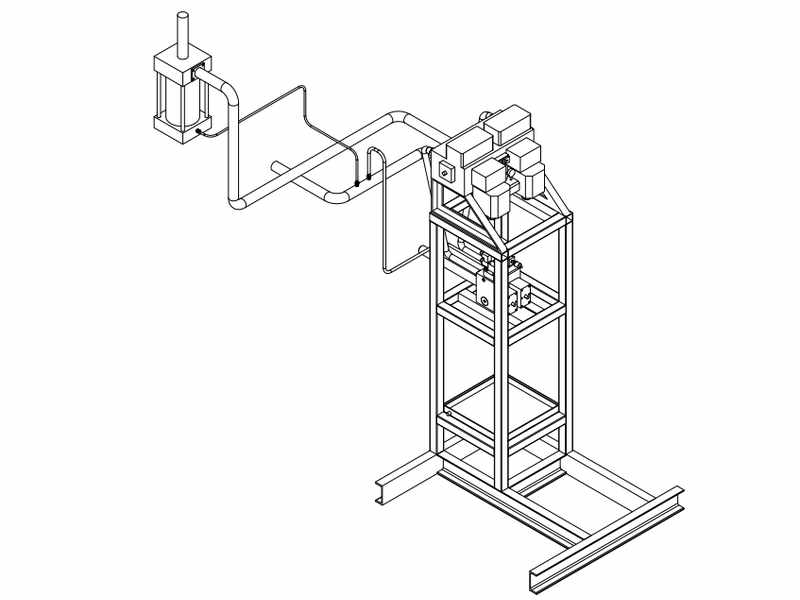
\includegraphics[angle=0,width=0.9\columnwidth]{install.jpg}
%\caption{安装支架及油路布置设计}
%\label{fig:install}
%\end{center}
%\end{figure}

冗余装置支架基础安装方面, 考虑到透平机组长时间运转,机组底座的振动大,所以没有把冗余装置安装到汽机底座,而是安装到建筑物平台上,并进行加固,保证系统的可靠性。
%\begin{figure}[H]
%\begin{center}
%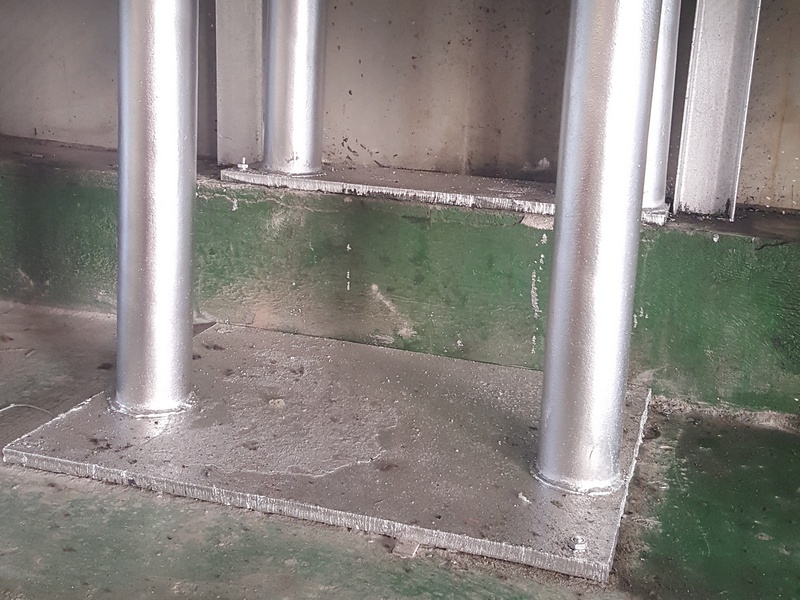
\includegraphics[angle=0,width=0.9\columnwidth]{base.jpg}
%\caption{冗余装置基础安装}
%\label{fig:base}
%\end{center}
%\end{figure}

油缸位置反馈(MLDT)为控制系统提供精确的位置反馈,同时要经受长期的机组本体振动,所以安装的精度和可靠性要求也很高。改造方案专门设计了MLDT安装支架,精确配合机组油缸和拉杆位置,保证改造后的控制精度和可靠性,如图\ref{fig:mldt_install}所示。\par
除上述方面,安装过程还考虑了如油路清洁等多方面因素,进行管道清洗等。改造前后的机组外观如图\ref{fig:turbine_before} 和图\ref{fig:turbine_after}所示。\par
\begin{figure}[H]
\begin{center}
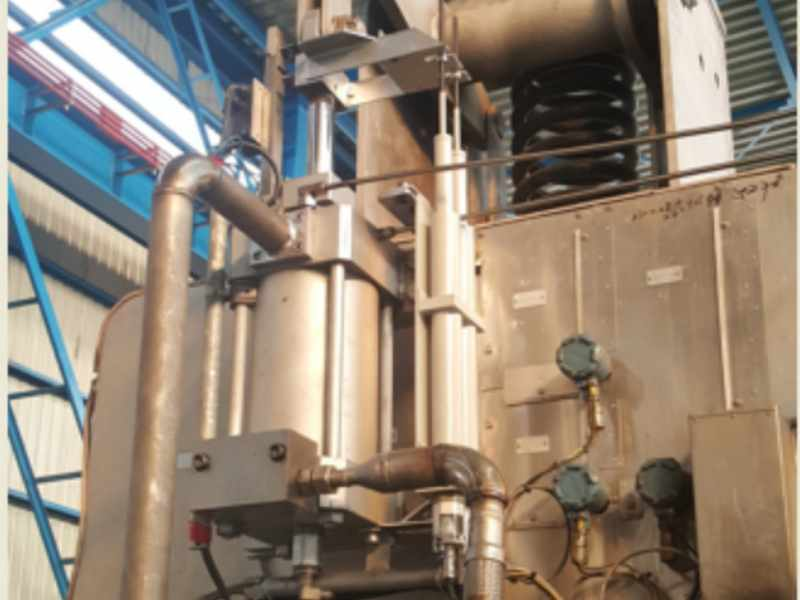
\includegraphics[angle=0,width=0.9\columnwidth]{mldt_install.jpg}
\caption{油缸位置反馈装置的安装}
\label{fig:mldt_install}
\end{center}
\end{figure}
\section*{改造结果}
%\raggedbottom
改造后的系统经过静态和动态试验, 实现了控制信号、伺服阀、MLDT位置传感器、供电电源任一部件故障不停机、并且两路伺服控制可以无扰切换和部件在线热替换, 彻底消除了系统的单点环节, 实现了设计要求, 试验数据见表\ref{table:result}和图\ref{fig:curve}。改造后的机组于2017年12月15日正式投入运行并带负荷向高炉送风,投入实际生产,至今运行良好。\par 
梅钢新三号机的伺服系统冗余的成功改造有两点重要意义。\par
首先,改造后的伺服系统彻底消除了原来系统的单点环节,实现了电液伺服阀、反馈装置、指令信号和供电系统任一部件故障不停机,提高了系统的可靠性,为梅山钢铁的安全生产做出了贡献。\par
其次,即使在世界范围内,实现彻底的伺服驱动冗余的项目也不多,在国内更是鲜有耳闻。梅钢新三号机的项目的成功,为探索伺服驱动环节冗余,提高机组可靠性,积累了第一手的宝贵工程经验, 无论是对钢铁和石化领域动力机组最终用户还是对透平制造商都有重大的借鉴意义。\par
\end{multicols}
\begin{center}
\noindent
\begin{minipage}[c]{0.48\textwidth}
\begin{figure}[H]
\begin{center}
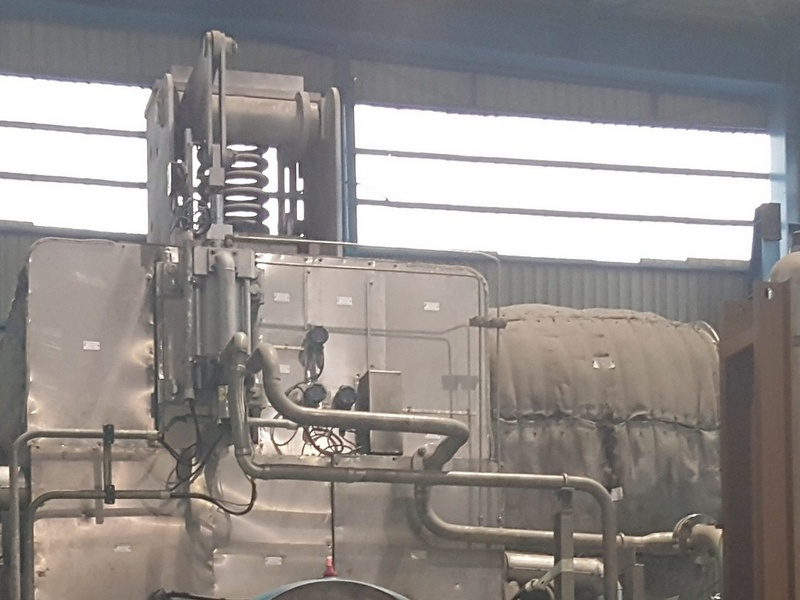
\includegraphics[angle=0,width=\columnwidth]{turbine_before.jpg}
\caption{改造前的机组}
\label{fig:turbine_before}
\end{center}
\end{figure}
\end{minipage}
\hfill
\begin{minipage}[c]{0.48\textwidth}
\begin{figure}[H]
\begin{center}
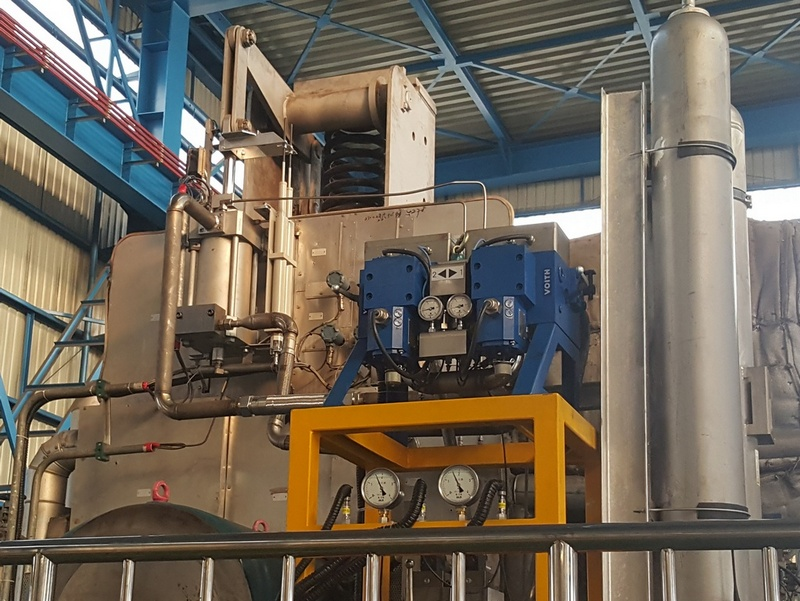
\includegraphics[angle=0,width=\columnwidth]{turbine_after.jpg}
\caption{改造后的机组}
\label{fig:turbine_after}
\end{center}
\end{figure}
\end{minipage}
\end{center}		


\begin{table}[H]
\renewcommand\arraystretch{1.2}
\begin{center}
\begin{tabular}{|>{\centering}p{0.22\textwidth}|>{\centering}p{0.18\textwidth}|>{\centering}p{0.1\textwidth}|>{\centering}p{0.18\textwidth}|>{\centering}p{0.1\textwidth}|}
\hline
\multirow{2}{*}{试验项目}& \multicolumn{2}{c|}{切换前} & \multicolumn{2}{c|}{切换后}  \tabularnewline
\cline{2-5}
& 控制油压(KPa) & 阀位(\%) & 控制油压(KPa) & 阀位(\%) \tabularnewline
\hline
Voith阀A失电 & 442 & 50 & 448 & 50 \tabularnewline
\hline
Voith阀B失电 & 445 & 50 & 443 & 50 \tabularnewline
\hline
控制指令A故障 & 443 & 50 & 448 & 50 \tabularnewline
\hline
控制指令B故障 & 441 & 50 & 437 & 50 \tabularnewline
\hline
MLDT信号A故障 & 448 & 50 & 439 & 50 \tabularnewline
\hline
MLDT信号B故障 & 440 & 50 & 439 & 50 \tabularnewline
\hline
手动切除A路位阀 & 441 & 50 & 448 & 50 \tabularnewline
\hline
手动切除B路位阀 & 446 & 50 & 442 & 50 \tabularnewline
\hline
监控系统失电 & 444 & 50 & 443 & 50 \tabularnewline
\hline
\end{tabular}
\caption{冗余试验结果}
\label{table:result}
\end{center}
\end{table}

\begin{figure}[H]
\begin{center}
	\begin{tikzpicture}[scale=1]
	\begin{axis}[
			width=13cm, 
			height=6.5cm, 
			tick align=inside, 
			xlabel={阀位指令[mA]}, 
			ylabel={油动机行程[mm]},
			xmin=0, 
			xmax=20, 
			ymin=0, 
			ymax=200, 
			grid style=dashed,
			xtick={0, 4, 8, 12, 16, 20},
			ytick={0, 50, 100, 150, 200},
			ymajorgrids=true,
			legend pos=north west,
			]
		\addplot[color=blue,mark=square] coordinates {(4,10) (5.6,25) (7.2,45) (8.8,65) (10.4,85) (12,105) (13.6,120) (15.2,135) (16.8,155) (18.4,175) (20,195)};
		\addlegendentry{改造后调门曲线} 
	\end{axis}
\end{tikzpicture}
\caption{改造后的调门曲线 Test Test}
\label{fig:curve}
\end{center}
\end{figure}

\begin{tikzpicture}[remember picture,overlay]
\fill[titleblue1] (current page.south west) rectangle ([yshift=0.05\paperheight]current page.south east);%底部蓝色背景
\end{tikzpicture}
%\begin{multicols}{2}
\end{document}
